\documentclass[11pt]{beamer}
\usepackage[T2A]{fontenc}
\usepackage[utf8]{inputenc}
\usepackage[english,russian]{babel}
\usepackage{amssymb,amsfonts,amsmath,mathtext, mathtools}
\usepackage{cite,enumerate,float,indentfirst}
\usepackage{subcaption}

\graphicspath{{images/}}

\usetheme[usetitleprogressbar, usetotalslideindicator, nooffset]{m}

%%% Переопределение именований %%%

\newcommand{\tr}{\mathrm{Tr}}
\newcommand{\e}{\mathrm{e}}
\renewcommand{\imath}{\mathrm{i}}

\newcommand{\N}{\mathbb{N}}
\newcommand{\Z}{\mathbb{Z}}
\newcommand{\R}{\mathbb{R}}
\newcommand{\exR}{\overline{\mathbb{R}}}
\renewcommand{\P}{\mathbb{P}}
\renewcommand{\C}{\mathbb{C}}

\newcommand{\J}{\mathcal{J}}

\renewcommand{\leq}{\leqslant}
\renewcommand{\geq}{\geqslant}

\renewcommand{\Re}{\mathop{\mathrm{Re}}\nolimits}
\renewcommand{\Im}{\mathop{\mathrm{Im}}\nolimits}

\renewcommand{\d}{\mathrm{d}}

\newcommand{\dd}[2]{\frac{\d{#1}}{\d{#2}}}
\newcommand{\ddd}[2]{\frac{\d^2{#1}}{\d{#2}^2}}
\newcommand{\pd}[2]{\frac{\partial{#1}}{\partial{#2}}}
\newcommand{\pdd}[2]{\frac{\partial^2{#1}}{\partial{#2}^2}}
\newcommand{\pdp}[3]{\frac{\partial^2{#1}}{\partial{#2}\partial{#3}}}
\newcommand{\pdet}[1]{\det\left({#1}\right)}
\renewcommand{\exp}[1]{\mathrm{e}^{#1}}
\newcommand{\half}[1]{\frac{#1}{2}}

\newcommand{\trans}[1]{{#1}^\mathrm{T}}
\newcommand{\op}[1]{\mathrm{#1}}

\newcommand{\E}{\op{E}}
\newcommand{\D}{\op{D}}
\newcommand{\cov}{\op{cov}}
\newcommand{\Dom}{\op{Dom}}
\newcommand{\Ran}{\op{Ran}}

\newcommand*\Diff{\mathop{}\!\mathbin\bigtriangleup}
\DeclarePairedDelimiter\brts{(}{)}
\DeclarePairedDelimiter\sqts{[}{]}
           % Переопределение именований

\title{\small{Институт прикладной математики и механики, СПбГПУ\\%
Изучение связей между оценками параметров моделей случайных процессов с помощью копул}}
\author{\small{%
Выступающий ст. гр. 43601/2: \hfill ~И. П. Дмитриевский\\%
Руководитель:~доц.,~к.ф.-м.н. \hfill ~А. А. Иванков}\\%
\vfill
}
\date{\small{Санкт-Петербург, 2015}}

\begin{document}

\maketitle

\begin{frame}
\frametitle{Модель случайного процесса}
\begin{equation}
X(t) = Z(t) + Y(t)
\end{equation}
\begin{equation}
Z(t) = \mu + \sigma W(t)
\end{equation}
\begin{equation}
Y(t) = \sum_{j=0}^K P_j \cdot I(t - \tau_j) \cdot e^{-\lambda_c(t - \tau_j)}
\end{equation}
\begin{equation}
(\mu, \sigma, x_m, \alpha, \lambda, \lambda_c)
\end{equation}
\end{frame}

\begin{frame}
\frametitle{Оценивание параметров $X(t)$}
\begin{itemize}
  \item Реализован алгоритм оценивания параметров процесса (Сидоровская, 2015 г.);
  \item В рамках реализованного подхода наиболее критичный этап --- интервальное оценивание;
\end{itemize}
\end{frame}

\begin{frame}
\frametitle{Постановка задачи}
Дано:
\begin{itemize}
  \item Результаты вычислительных экспериментов по интервальному оцениванию (Сидоровская, 2015 г.);
  \item Величина набора данных $\sim 10^5$;
\end{itemize}

Требуется:
\begin{itemize}
  \item Оценить стохастические связи между модельными значениями параметров и результатами алгоритма интервального оценивания;
\end{itemize}
\end{frame}

\begin{frame}
\frametitle{Выбранный метод}
\begin{itemize}
  \item Различные коэффициенты корреляции дают слабое представление о структуре связи;
  \item Для более полного изучения связей требуется аппроксимировать двумерное распределение;
  \item Копулы дают исчерпывающее описание стохастической связи;
\end{itemize}
\end{frame}

\begin{frame}
\begin{center}
\frametitle{Копулы}
\begin{equation}
H(x, y) = C(F(x), G(y))
\end{equation}
\begin{itemize}
  \item Аппарат копул молод и активно развивается;
  \item Копулы успешно применяются во многих сферах;
  \item Копулы являются гибким инструментом для исследования связей;
\end{itemize}
\end{center}
\end{frame}

\begin{frame}
\begin{center}
\frametitle{Выяснение связей между параметрами}
\begin{itemize}
  \item Собран набор данных вида (модельная шестёрка параметров; количество параметров, попавших в оценённый по этой шестёрке компакт);
  \item Отбираются те пары, для которых количество попавших параметров не меньше какого-то значения, например, пяти;
  \item Строится шестимерная копула на основе получившегося набора левых частей отобранных пар;
  \item Строятся двумерные проекции этой копулы для оценки связи различных пар параметров;
  \item Делается вывод о том, какие соотношения параметров приводят к провалу алгоритма;
\end{itemize}
\end{center}
\end{frame}


\begin{frame}
\begin{center}
Спасибо за внимание!
\end{center}
\end{frame}

\begin{frame}
\frametitle{Пуассоновский поток событий $Y(t)$}
\[Y(t) = \sum_{j = 0}^K P_j \cdot I(t - \tau_j) \cdot e^{-\lambda_c(t - \tau_j)}\]
\begin{itemize}
  \item $K$~---~число событий, поступивших до момента $t$;
  \item $\tau_j$~---~время возникновения $j$-ого возмущения;
  \item $I$~---~функция Хевисайда;
  \item $\lambda_c$~---~константа, одинаковая для всех событий;
  \item $P_j$~---~случайная величина, распределённая по закону Парето с параметрами $x_m$ и $\alpha$, одинаковыми для всех событий:
\[
f_{P_j}(x) = \begin{cases}
\frac{\alpha x_m^\alpha}{x^{\alpha+1} }, &x \geqslant x_m,\\
0, &x < x_m.
\end{cases}
\]
\end{itemize}
\end{frame}

\begin{frame}
\frametitle{Метод отражений}
\[\hat{c}_h(u, v) = \frac{1}{Th^2}\sum_{i=1}^T\sqts{K\brts{\frac{u - \hat{U}_i}{h}}K\brts{\frac{v - \hat{V}_i}{h}} + \cdots},\]
где места $\hat{U}_i$ и $\hat{V}_i$ занимают все отражения $(\pm\hat{U}_i, \pm\hat{V}_i), (\pm\hat{U}_i, 2 - \hat{V}_i), (2- \hat{U}_i, \pm\hat{V}_i), (2 - \hat{U}_i, 2- \hat{V}_i)$.
\end{frame}

\begin{frame}
\frametitle{Метод преобразований}
\begin{align}
\hat{c}_h(u, v) = &\frac{1}{Th^2g(G^{-1}(u))g(G^{-1}(v))}\times \\
&\sum_{i=1}^T K\brts{\frac{G^{-1}(u) - G^{-1}(\hat{U}_i)}{h},\frac{G^{-1}(v) - G^{-1}(\hat{V}_i)}{h}}
\end{align}
где $G$ --- функция распределения с положительной плотностью $g$.
\end{frame}

\begin{frame}
\frametitle{Копулы}
\emph{Двумерной копулой} называется функция $C$, удовлетворяющая следующим свойствам:
\begin{enumerate}
\item $\Dom{C} = I^2$;
\item $\forall u,v \in I : C(u, 0) = 0 = C(0, v)$;
\item $\forall B = [x_1, x_2] \times [y_1, y_2] \subset I^2 : \Diff_{y_1}^{y_2}\Diff_{x_1}^{x_2}C(x, y) \geqslant 0$;
\item Для каждых $u, v \in I$:
  \begin{gather}
    C(u, 1) = u \\
    C(1, v) = v.
  \end{gather}
\end{enumerate}
\end{frame}

\begin{frame}
\frametitle{Примеры копул}
\begin{figure}[H]
  \centering
  \begin{subfigure}{.3\textwidth}
    \centering
    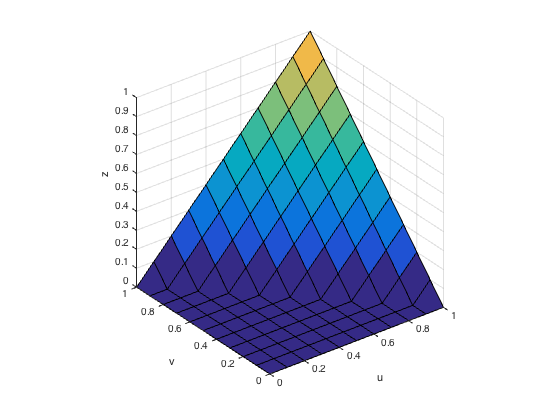
\includegraphics[width=\linewidth]{W.png}
    \caption{$z = W(u, v)$}
  \end{subfigure}%
  \begin{subfigure}{.3\textwidth}
    \centering
    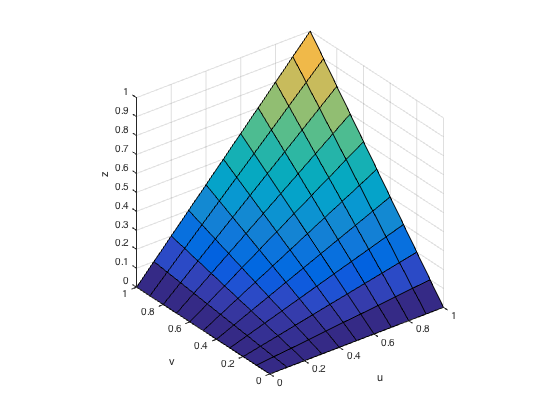
\includegraphics[width=\linewidth]{P.png}
    \caption{$z = P(u, v)$}
  \end{subfigure}
  \begin{subfigure}{.3\textwidth}
    \centering
    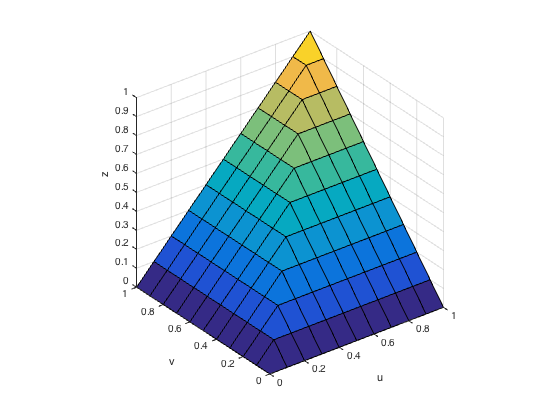
\includegraphics[width=\linewidth]{M.png}
    \caption{$z = M(u, v)$}
  \end{subfigure}
  \caption{Графики копул $W$, $P$ и $M$}
\end{figure}
\end{frame}

\begin{frame}
\frametitle{Теорема Скляра и теорема об инвариантности}
\begin{itemize}
\item Пусть $X, Y$ --- случайные величины с распределениями $F, G$ соответственно, и совместным распределением $H$. Тогда выполняется уравнение
\begin{equation}
  H(x, y) = C(F(x), G(y)).
\end{equation}
Если $F$ и $G$ непрерывны, то $C$ единственна;

\item Пусть $X, Y$ --- непрерывные случайные величины c копулой $C_{XY}$. Если $\alpha$ и $\beta$ строго возрастают на $\Ran{X}$ и $\Ran{Y}$ соответственно, то $C_{\alpha(X)\beta(Y)} = C_{XY}$. Таким образом $C_{XY}$ инвариантна относительно строго возрастающих преобразований $X$ и $Y$.
\end{itemize}
\end{frame}

\begin{frame}
\frametitle{Коэффициент корреляции Пирсона}
\begin{figure}\label{fig:pearson}
\centering
\begin{subfigure}{.45\textwidth}
  \centering
  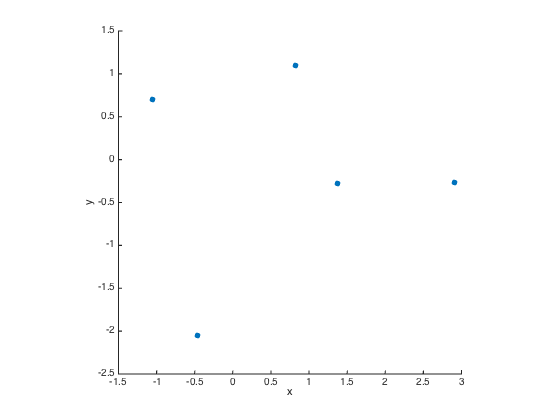
\includegraphics[width = \textwidth]{./images/normscatter.png}
  \caption{$(x, y) \sim \mathcal{N}, \rho = 0.06 $}
  \label{fig:norm}
\end{subfigure}
\begin{subfigure}{.45\textwidth}
  \centering
  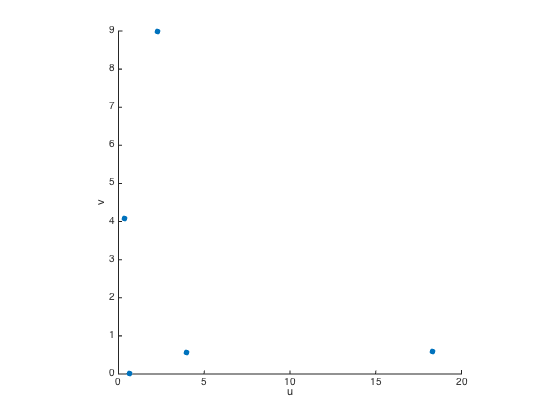
\includegraphics[width = \textwidth]{./images/transformed_normscatter.png}
  \caption{$(x, y) = (\e^x, \e^{2y}), \rho = -0.33$}
  \label{fig:transnorm}
\end{subfigure}
\end{figure}
\end{frame}

\begin{frame}
\frametitle{Коэффициент ранговой корреляции Кендалла}
\begin{itemize}
  \item \emph{Коэффициентом ранговой корреляции} вектора случайных величин $\trans{(X, Y)}$ называется величина
\begin{equation}
  \tau(X, Y) = \P\{\, (X - \widetilde{X})(Y - \widetilde{Y}) > 0 \,\} - \P\{\, (X - \widetilde{X})(Y - \widetilde{Y}) < 0 \,\},
\end{equation}
где $\trans{(\widetilde{X}, \widetilde{Y})}$ --- независимая копия $\trans{(X, Y)}$. \par

\item Пусть $X, Y$ --- непрерывные случайные величины с копулой $C$, тогда их коэффициенту Кендалла соответствует выражение
  \[
  \tau(X, Y) = \tau_C = 4 \iint_{I^2} C(u, v) \d C(u,v) - 1.
  \]
\end{itemize}
\end{frame}

\begin{frame}
\begin{center}
\frametitle{Построение эмпирических копул}
\begin{figure}[H]
  \centering
  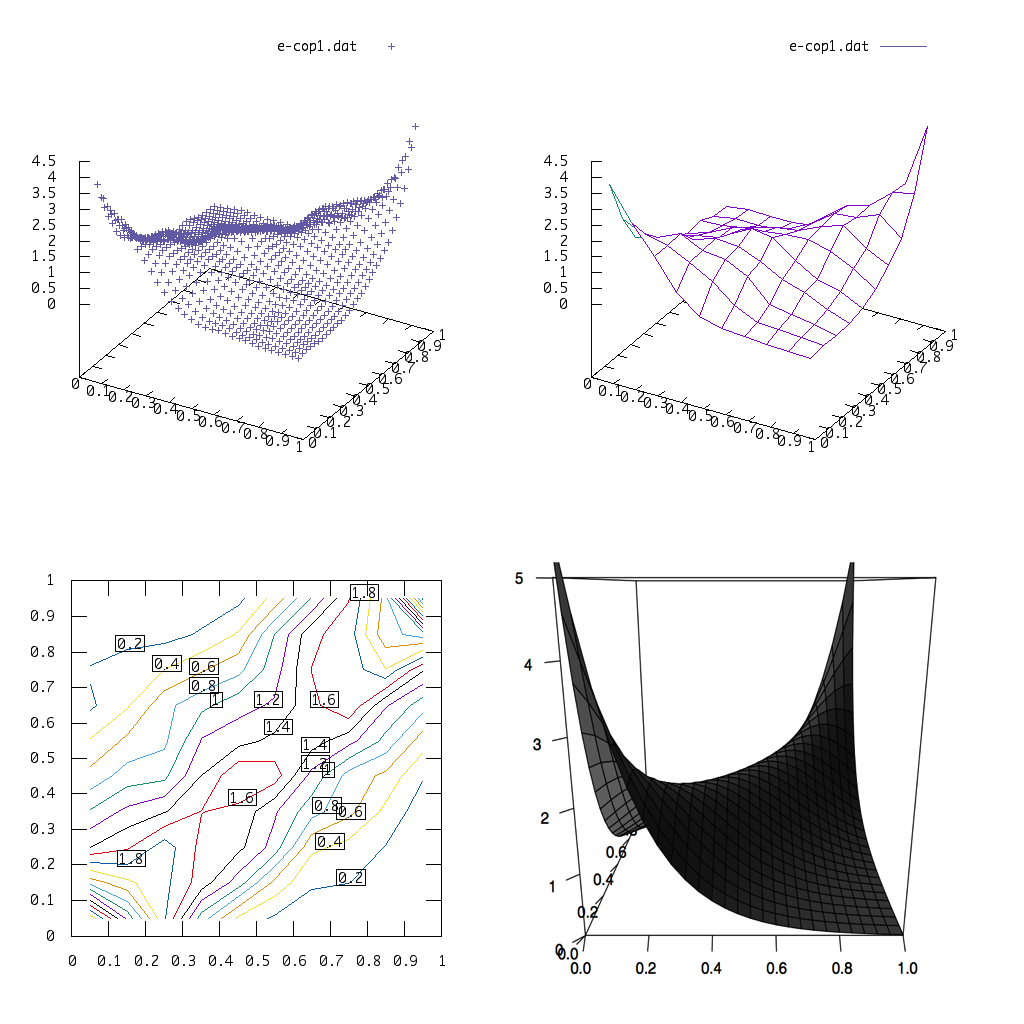
\includegraphics[width=.56\textwidth]{FrankMirror.png}
  \caption{Графики оценённой (метод отражений, 1000 наблюдений) и истинной плотностей копулы Фрэнка}
\end{figure}
\end{center}
\end{frame}

\begin{frame}
\begin{center}
\frametitle{Построение эмпирических копул (1)}
\begin{figure}[H]
  \centering
  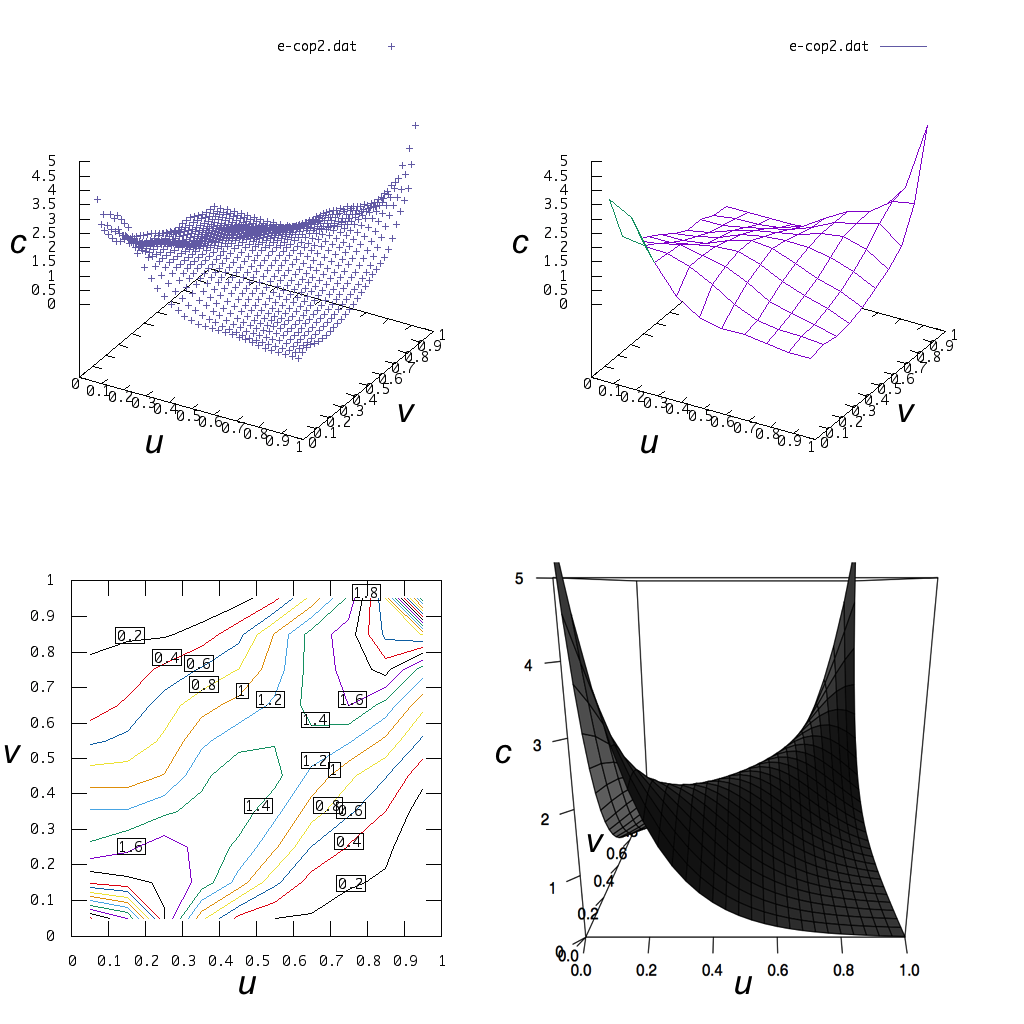
\includegraphics[width=.56\textwidth]{FrankTransform.png}
  \caption{Графики оценённой (метод преобразований, 1000 наблюдений) и истинной плотностей копулы Фрэнка}
\end{figure}
\end{center}
\end{frame}

\end{document}
